\section{Training the Generative Model}
\label{sec:training_generative_models}
In the last two sections, we showed how to construct a generative model with a vector field $u_t^\theta$ given by a neural network, and we derived a formula for the training target $\uref_t$. In this section, we will describe how to train the neural network $u_t^\theta$ to approximate the training target $\uref_t$. First, we restrict ourselves to ODEs again, in doing so recovering \themebf{flow matching}. Second, we explain how to extend the approach to SDEs via \themebf{score matching}. Finally, we consider the special case of Gaussian probability paths, in doing so recovering \themebf{denoising diffusion models}. With these tools, we will at last have an end-to-end procedure to train and sample from a generative model with ODEs and SDEs.

在前两个章节中,我们展示了如何用神经网络构建带有向量场 $u_t^\theta$ 的生成模型,并推导出了训练目标 $\uref_t$ 的公式。在本节中,我们将描述如何训练神经网络 $u_t^\theta$ 来近似训练目标 $\uref_t$。首先,我们再次限制自己使用常微分方程,从而恢复\themebf{流匹配(flow matching)}。其次,我们解释如何通过\themebf{分数匹配(score matching)}将方法扩展到随机微分方程。最后,我们考虑高斯概率路径的特殊情况,从而恢复\themebf{去噪扩散模型(denoising diffusion models)}。有了这些工具,我们最终将拥有一个端到端的程序来训练生成模型并从 ODE 和 SDE 中采样。

\subsection{Flow Matching}

As before, let us consider a flow model given by
\begin{align}
\label{eq:ode_model}
 X_0&\sim\pinit,\quad \dd X_t = u_t^\theta(X_t)\,\dd t. &&\blacktriangleright\,\,\text{flow model/流模型}
\end{align}
As we learned, we want the neural network $u_t^\theta$ to equal the marginal vector field $\uref_t$. In other words, we would like to find parameters $\theta$ so that $u_t^\theta\approx \uref_t$. In the following, we denote by $\text{Unif}=\text{Unif}_{[0,1]}$ the uniform distribution on the interval $[0,1]$, and by $\mathbb{E}$ the expected value of a random variable. An intuitive way of obtaining $u_t^\theta\approx \uref_t$ is to use a mean-squared error, i.e. to use the \themebf{flow matching loss} defined as

如前所述,让我们考虑一个由下式给出的流模型:
\begin{align}
\label{eq:ode_model}
 X_0&\sim\pinit,\quad \dd X_t = u_t^\theta(X_t)\,\dd t. &&\blacktriangleright\,\,\text{flow model/流模型}
\end{align}
正如我们所学的,我们希望神经网络 $u_t^\theta$ 等于边际向量场 $\uref_t$。换句话说,我们希望找到参数 $\theta$ 使得 $u_t^\theta\approx \uref_t$。在下文中,我们用 $\text{Unif}=\text{Unif}_{[0,1]}$ 表示区间 $[0,1]$ 上的均匀分布,用 $\mathbb{E}$ 表示随机变量的期望值。获得 $u_t^\theta\approx \uref_t$ 的一种直观方法是使用均方误差,即使用定义为下式的\themebf{流匹配损失(flow matching loss)}:
\label{subsec:training_algorithm}
\begin{align}
    \label{eq:marginal_loss_function}
\Lmarg(\theta)&=\mathbb{E}_{t\sim\text{Unif},x\sim p_t}[\|u_t^\theta(x) - \uref_t(x)\|^2]\\&\overset{(i)}{=} \mathbb{E}_{t\sim\text{Unif},z\sim \pdata, x\sim p_t(\cdot|z)}[\|u_t^\theta(x) - \uref_t(x)\|^2],
\end{align}
where $p_t(x)=\int p_t(x|z)\pdata(z) \dd z$ is the marginal probability path and in $(i)$ we used the sampling procedure given by \cref{eq:marginal_prob_path}. Intuitively, this loss says: First, draw a random time $t \in [0,1]$. Second, draw a random point $z$ from our data set, sample from $p_t(\cdot|z)$ (e.g., by adding some noise), and compute $u_t^\theta(x)$. Finally, compute the mean-squared error between the output of our neural network and the marginal vector field $\uref_t(x)$. Unfortunately, we are \textit{not} done here. While we do know the formula for $\uref_t$ by \cref{thm:marginalization_trick}
\begin{align}
\label{eq:marginal_vector_field_stated_again}
    \uref_t(x) = \int \uref_t(x|z)\frac{ p_t(x|z)\pdata(z)}{p_t(x)}\dd z,
\end{align}
we cannot compute it efficiently because the above integral is intractable. Instead, we will exploit the fact that the \themebf{conditional} velocity field $\uref_t(x|z)$ is tractable. % We could try to approximate the above integral by screening over the whole dataset. However, even for a dataset of 1 million images (which is very small in modern days), we would need to loop over 1 million images every time we evaluate $\uref_t(x)$ - an extremely computationally expensive approach. However, it turns out that we can solve this. 

其中 $p_t(x)=\int p_t(x|z)\pdata(z) \dd z$ 是边际概率路径,在 $(i)$ 中我们使用了\cref{eq:marginal_prob_path}给出的采样过程。直观地说,这个损失的含义是:首先,随机抽取时间 $t \in [0,1]$。其次,从数据集中随机抽取一个点 $z$,从 $p_t(\cdot|z)$ 中采样(例如,通过添加一些噪声),并计算 $u_t^\theta(x)$。最后,计算神经网络输出与边际向量场 $\uref_t(x)$ 之间的均方误差。不幸的是,我们在这里还\textit{没有}完成。虽然我们通过\cref{thm:marginalization_trick}知道了 $\uref_t$ 的公式
\begin{align}
\label{eq:marginal_vector_field_stated_again}
    \uref_t(x) = \int \uref_t(x|z)\frac{ p_t(x|z)\pdata(z)}{p_t(x)}\dd z,
\end{align}
但我们无法有效地计算它,因为上述积分是难以处理的。相反,我们将利用\themebf{条件}速度场 $\uref_t(x|z)$ 是可处理的这一事实。 

To do so, let us define the \themebf{conditional flow matching loss} 
\begin{align}
\label{eq:cfm}
\Lcond(\theta) =     \mathbb{E}_{t\sim \Unif, z\sim \pdata, x\sim p_t(\cdot|\dap)}[\|u_t^\theta(x) - \uref_t(x|\dap)\|^2].
\end{align}
Note the difference to     \cref{eq:marginal_loss_function}: we use the conditional vector field $\uref_t(x|z)$ instead of the marginal vector $\uref_t(x)$. As we have an analytical formula for $\uref_t(x|z)$, we can minimize the above loss easily. But wait, what sense does it make to regress against the conditional vector field if it's the marginal vector field we care about? As it turns out, by \themeit{explicitly} regressing against the tractable, conditional vector field, we are \themeit{implicitly} regressing against the intractable, marginal vector field. The next result makes this intuition precise.

为此,让我们定义\themebf{条件流匹配损失(conditional flow matching loss)}:
\begin{align}
\label{eq:cfm}
\Lcond(\theta) =     \mathbb{E}_{t\sim \Unif, z\sim \pdata, x\sim p_t(\cdot|\dap)}[\|u_t^\theta(x) - \uref_t(x|\dap)\|^2].
\end{align}
注意与\cref{eq:marginal_loss_function}的区别:我们使用条件向量场 $\uref_t(x|z)$ 而不是边际向量场 $\uref_t(x)$。由于我们有 $\uref_t(x|z)$ 的解析公式,我们可以轻松地最小化上述损失。但是等等,如果我们关心的是边际向量场,那么对条件向量场进行回归有什么意义呢?事实上,通过\themeit{显式地}对可处理的条件向量场进行回归,我们实际上是在\themeit{隐式地}对难以处理的边际向量场进行回归。下一个结果使这种直觉变得精确。

\begin{theorem}
\label{thm:fm_loss} 
The marginal flow matching loss equals the conditional flow matching loss up to a constant. That is,

边际流匹配损失等于条件流匹配损失加上一个常数。即,

\begin{align*}
\Lmarg(\theta) = \Lcond(\theta) + C,
\end{align*}

where $C$ is independent of $\theta$. Therefore, their gradients coincide:

其中 $C$ 与 $\theta$ 无关。因此,它们的梯度重合:

\begin{align*}
\nabla_\theta \Lmarg(\theta) = \nabla_\theta \Lcond(\theta).
\end{align*}

Hence, minimizing $\Lcond(\theta)$ with e.g., stochastic gradient descent (SGD) is equivalent to minimizing $\Lmarg(\theta)$ with in the same fashion. In particular, for the minimizer $\theta^*$ of $\Lcond(\theta)$, it will hold that $u_t^{\theta^*}=\uref_t$ (assuming an infintely expressive parameterization). 

因此,使用例如随机梯度下降(SGD)最小化 $\Lcond(\theta)$ 等价于以同样的方式最小化 $\Lmarg(\theta)$。特别地,对于 $\Lcond(\theta)$ 的最小化器 $\theta^*$,将有 $u_t^{\theta^*}=\uref_t$(假设具有无限表达能力的参数化)。
\end{theorem}
\begin{proof}
The proof works by expanding the mean-squared error into three components and removing constants:
\begin{align*}
    \Lmarg(\theta)&\overset{(i)}{=}\mathbb{E}_{t\sim\text{Unif},x\sim p_t}[\|u_t^\theta(x) - \uref_t(x)\|^2]\\
    &\overset{(ii)}{=}\mathbb{E}_{t\sim\text{Unif},x\sim p_t}[\|u_t^\theta(x)\|^2 - 2u_t^\theta(x)^T\uref_t(x) + \|\uref_t(x)\|^2]\\
    &\overset{(iii)}{=}\mathbb{E}_{t\sim\text{Unif},x\sim p_t}\left[\|u_t^\theta(x)\|^2\right] - 2\mathbb{E}_{t\sim\text{Unif},x\sim p_t}[u_t^\theta(x)^T\uref_t(x)] + \underbrace{\mathbb{E}_{t\sim\text{Unif}_{[0,1]}, x\sim p_t}[\|\uref_t(x)\|^2]}_{=:C_1}\\
    &\overset{(iv)}{=}\mathbb{E}_{t\sim\text{Unif},z\sim\pdata, x\sim p_t(\cdot|z)}[\|u_t^\theta(x)\|^2] - 2\mathbb{E}_{t\sim\text{Unif},x\sim p_t}[u_t^\theta(x)^T\uref_t(x)] + C_1
\end{align*}
where $(i)$ holds by definition, in $(ii)$ we used the formula $\|a-b\|^2=\|a\|^2-2a^Tb+\|b\|^2$, in $(iii)$ we define a constant $C_1$ and in $(iv)$ we used the sampling procedure of $p_t$ given by \cref{eq:marginal_prob_path}. Let us reexpress the second summand:

证明通过将均方误差展开为三个分量并去除常数来进行:
\begin{align*}
    \Lmarg(\theta)&\overset{(i)}{=}\mathbb{E}_{t\sim\text{Unif},x\sim p_t}[\|u_t^\theta(x) - \uref_t(x)\|^2]\\
    &\overset{(ii)}{=}\mathbb{E}_{t\sim\text{Unif},x\sim p_t}[\|u_t^\theta(x)\|^2 - 2u_t^\theta(x)^T\uref_t(x) + \|\uref_t(x)\|^2]\\
    &\overset{(iii)}{=}\mathbb{E}_{t\sim\text{Unif},x\sim p_t}\left[\|u_t^\theta(x)\|^2\right] - 2\mathbb{E}_{t\sim\text{Unif},x\sim p_t}[u_t^\theta(x)^T\uref_t(x)] + \underbrace{\mathbb{E}_{t\sim\text{Unif}_{[0,1]}, x\sim p_t}[\|\uref_t(x)\|^2]}_{=:C_1}\\
    &\overset{(iv)}{=}\mathbb{E}_{t\sim\text{Unif},z\sim\pdata, x\sim p_t(\cdot|z)}[\|u_t^\theta(x)\|^2] - 2\mathbb{E}_{t\sim\text{Unif},x\sim p_t}[u_t^\theta(x)^T\uref_t(x)] + C_1
\end{align*}
其中 $(i)$ 根据定义成立,在 $(ii)$ 中我们使用了公式 $\|a-b\|^2=\|a\|^2-2a^Tb+\|b\|^2$,在 $(iii)$ 中我们定义了一个常数 $C_1$,在 $(iv)$ 中我们使用了\cref{eq:marginal_prob_path}给出的 $p_t$ 的采样过程。让我们重新表达第二个求和项:
\begin{align*}
\mathbb{E}_{t\sim\text{Unif},x\sim p_t}[u_t^\theta(x)^T\uref_t(x)]&\overset{(i)}{=}\int\limits_{0}^{1}\int p_t(x)u_t^\theta(x)^T\uref_t(x)\,\dd x\, \dd t\\
&\overset{(ii)}{=}\int\limits_{0}^{1}\int p_t(x)u_t^\theta(x)^T\left[\int \uref_t(x|z)\frac{ p_t(x|z)\pdata(z)}{p_t(x)}\dd z\right]\dd x\, \dd t\\
&\overset{(iii)}{=}\int\limits_{0}^{1}\int\int u_t^\theta(x)^T\uref_t(x|z) p_t(x|z)\pdata(z)\,\dd z\,\dd x\, \dd t\\
&\overset{(iv)}{=}\mathbb{E}_{t\sim\text{Unif},z\sim \pdata, x\sim p_t(\cdot|z)}[u_t^\theta(x)^T\uref_t(x|z)]
\end{align*}
where in $(i)$ we expressed the expected value as an integral, in $(ii)$ we use \cref{eq:marginal_vector_field_stated_again}, in $(iii)$ we use the fact that integrals are linear, in $(iv)$ we express the integral as an expected value. Note that this was really the crucial step of the proof: The beginning of the equality used the marginal vector field $\uref_t(x)$, while the end uses the conditional vector field $\uref_t(x|z)$. We plug is into the equation for $\Lmarg$ to get:

其中在 $(i)$ 中我们将期望值表示为积分,在 $(ii)$ 中我们使用\cref{eq:marginal_vector_field_stated_again},在 $(iii)$ 中我们使用积分的线性性质,在 $(iv)$ 中我们将积分表示为期望值。注意这确实是证明的关键步骤:等式的开始使用了边际向量场 $\uref_t(x)$,而结尾使用了条件向量场 $\uref_t(x|z)$。我们将其代入 $\Lmarg$ 的方程得到:
\begin{align*}
\Lmarg(\theta)&\overset{(i)}{=}\mathbb{E}_{t\sim\text{Unif},z\sim \pdata, x\sim p_t(\cdot|z)}[\|u_t^\theta(x)\|^2]-2\mathbb{E}_{t\sim\text{Unif},z\sim \pdata, x\sim p_t(\cdot|z)}[u_t^\theta(x)^T\uref_t(x|z)] +C_1\\
&\overset{(ii)}{=}\mathbb{E}_{t\sim\text{Unif},z\sim \pdata, x\sim p_t(\cdot|z)}[\|u_t^\theta(x)\|^2-2u_t^\theta(x)^T\uref_t(x|z)+\|\uref_t(x|z)\|^2-\|\uref_t(x|z)\|^2] +C_1\\
&\overset{(iii)}{=}\mathbb{E}_{t\sim\text{Unif},z\sim \pdata, x\sim p_t(\cdot|z)}[\|u_t^\theta(x)-\uref_t(x|z)\|^2]+\underbrace{\mathbb{E}_{t\sim\text{Unif},z\sim \pdata, x\sim p_t(\cdot|z)}[-\|\uref_t(x|z)\|^2]}_{C_2} +C_1\\
&\overset{(iv)}{=}\Lcond(\theta) + \underbrace{C_2+C_1}_{=:C}
\end{align*}
where in $(i)$ we plugged in the derived equation, in $(ii)$ we added and subtracted the same value,  in $(iii)$ we used the formula $\|a-b\|^2=\|a\|^2-2a^Tb+\|b\|^2$ again, and in $(iv)$ we defined a constant in $\theta$. This finishes the proof.
\end{proof}

其中在 $(i)$ 中我们代入了推导的方程,在 $(ii)$ 中我们加上并减去相同的值,在 $(iii)$ 中我们再次使用了公式 $\|a-b\|^2=\|a\|^2-2a^Tb+\|b\|^2$,在 $(iv)$ 中我们定义了一个关于 $\theta$ 的常数。这完成了证明。

Once $u_t^{\theta}$ has been trained, we may simulate the flow model
\begin{align}
\label{eq:sde_extension_restated}
    \dd X_t = u_t^\theta(X_t)\, \dd t,\quad\quad X_0\sim\pinit
\end{align}
via e.g., \cref{alg:sampling_flow_model} to obtain samples $X_1\sim \pdata$. This whole pipeline is called \themebf{flow matching} in the literature \citep{lipman2022flow, liu2022flow, albergo2023stochastic, lipman2024flow}. The training procedure is summarized in \cref{alg:training_fm_score_matching_gaussian_paths} and visualized in \cref{fig:fm_illustration_checkerboard}. Let us now instantiate the conditional flow matching loss for the choice of Gaussian probability paths:

一旦 $u_t^{\theta}$ 训练完成,我们可以通过例如\cref{alg:sampling_flow_model}来模拟流模型
\begin{align}
\label{eq:sde_extension_restated}
    \dd X_t = u_t^\theta(X_t)\, \dd t,\quad\quad X_0\sim\pinit
\end{align}
以获得样本 $X_1\sim \pdata$。这整个流程在文献中被称为\themebf{流匹配} \citep{lipman2022flow, liu2022flow, albergo2023stochastic, lipman2024flow}。训练过程在\cref{alg:training_fm_score_matching_gaussian_paths}中总结,并在\cref{fig:fm_illustration_checkerboard}中可视化。现在让我们为高斯概率路径的选择实例化条件流匹配损失:
\begin{examplebox}[Flow Matching for Gaussian Conditional Probability Paths]
Let us return to the example of Gaussian probability paths $p_t(\cdot|z)=\mathcal{N}(\alpha_t z; \beta_t^2 I_d)$, where we may sample from the conditional path via
\begin{align}
\label{eq:sampling_procedure_gaussian_path_restated_for_fm}
    \epsilon\sim\mathcal{N}(0,I_d)\quad 
    \Rightarrow\quad x_t = \alpha_t z + \beta_t \epsilon \sim \mathcal{N}(\alpha_tz,\beta_t^2I_d)=p_t(\cdot|z).
\end{align}
As we derived in \cref{eq:conditional_gaussian_vf}, the conditional vector field $\uref_t(x|z)$ is given by
\begin{align}
\label{e:marginal_vf_cond_score}
    \uref_t(x|z) =& \left(\dot{\alpha}_t-\frac{\dot{\beta}_t}{\beta_t}\alpha_t\right)z+\frac{\dot{\beta}_t}{\beta_t}x,
\end{align}
where $\dot{\alpha}_t=\partial_t\alpha_t$ and $\dot{\beta}_t=\partial_t\beta_t$ are the respective time derivatives. Plugging in this formula, the conditional flow matching loss reads
\begin{align*}
\Lcond(\theta) &= \mathbb{E}_{t\sim \text{Unif},z\sim \pdata, x\sim \mathcal{N}(\alpha_tz,\beta_t^2I_d)}[\lVert u_t^\theta(x)-\left(\dot{\alpha}_t-\frac{\dot{\beta}_t}{\beta_t}\alpha_t\right)z-\frac{\dot{\beta}_t}{\beta_t}x\rVert^2]\\&\overset{(i)}{=}\mathbb{E}_{t\sim\Unif,z\sim \pdata, \epsilon\sim \mathcal{N}(0,I_d)}[\|u_t^\theta(\alpha_tz+\beta_t\epsilon)-(\dot{\alpha}_tz+\dot{\beta}_t\epsilon)\|^2]
\end{align*}
where in $(i)$ we plugged in \cref{eq:sampling_procedure_gaussian_path_restated_for_fm} and replaced $x$ by $\alpha_tz+\beta_t\epsilon$. Note the simplicity of $\Lcond$ : We sample a data point $z$, sample some noise $\epsilon$ and then we take a mean squared error. Let us make this even more concrete for the special case of $\alpha_t=t$, and $\beta_t=1-t$. The corresponding probability $p_t(x|z)=\mathcal{N}(tz,(1-t)^2)$ is sometimes referred to as the (Gaussian) \themebf{CondOT probability path}. Then we have $\dot{\alpha}_t=1,\dot{\beta}_t=-1$, so that
\begin{align*}
        \mathcal{L}_{\text{cfm}}(\theta)=&\mathbb{E}_{t\sim\Unif,z\sim \pdata, \epsilon\sim \mathcal{N}(0,I_d)}[\|u_t^\theta(tz+(1-t)\epsilon)-(z-\epsilon)\|^2]
\end{align*}
Many famous state-of-the-art models have been trained using this simple yet effective procedure, e.g. \themeit{Stable Diffusion 3}, Meta's \themeit{Movie Gen Video}, and probably many more proprietary models. In \cref{fig:fm_illustration_checkerboard}, we visualize it in a simple example and in \cref{alg:training_fm_score_matching_gaussian_paths} we summarize the training procedure.

让我们回到高斯概率路径 $p_t(\cdot|z)=\mathcal{N}(\alpha_t z; \beta_t^2 I_d)$ 的例子,我们可以通过以下方式从条件路径中采样:
\begin{align}
\label{eq:sampling_procedure_gaussian_path_restated_for_fm}
    \epsilon\sim\mathcal{N}(0,I_d)\quad 
    \Rightarrow\quad x_t = \alpha_t z + \beta_t \epsilon \sim \mathcal{N}(\alpha_tz,\beta_t^2I_d)=p_t(\cdot|z).
\end{align}
正如我们在\cref{eq:conditional_gaussian_vf}中推导的,条件向量场 $\uref_t(x|z)$ 由下式给出:
\begin{align}
\label{e:marginal_vf_cond_score}
    \uref_t(x|z) =& \left(\dot{\alpha}_t-\frac{\dot{\beta}_t}{\beta_t}\alpha_t\right)z+\frac{\dot{\beta}_t}{\beta_t}x,
\end{align}
其中 $\dot{\alpha}_t=\partial_t\alpha_t$ 和 $\dot{\beta}_t=\partial_t\beta_t$ 分别是对时间的导数。将此公式代入,条件流匹配损失为:
\begin{align*}
\Lcond(\theta) &= \mathbb{E}_{t\sim \text{Unif},z\sim \pdata, x\sim \mathcal{N}(\alpha_tz,\beta_t^2I_d)}[\lVert u_t^\theta(x)-\left(\dot{\alpha}_t-\frac{\dot{\beta}_t}{\beta_t}\alpha_t\right)z-\frac{\dot{\beta}_t}{\beta_t}x\rVert^2]\\&\overset{(i)}{=}\mathbb{E}_{t\sim\Unif,z\sim \pdata, \epsilon\sim \mathcal{N}(0,I_d)}[\|u_t^\theta(\alpha_tz+\beta_t\epsilon)-(\dot{\alpha}_tz+\dot{\beta}_t\epsilon)\|^2]
\end{align*}
其中在 $(i)$ 中我们代入了\cref{eq:sampling_procedure_gaussian_path_restated_for_fm}并用 $\alpha_tz+\beta_t\epsilon$ 替换了 $x$。注意 $\Lcond$ 的简单性:我们采样一个数据点 $z$,采样一些噪声 $\epsilon$,然后计算均方误差。让我们进一步具体化 $\alpha_t=t$ 和 $\beta_t=1-t$ 的特殊情况。相应的概率 $p_t(x|z)=\mathcal{N}(tz,(1-t)^2)$ 有时被称为(高斯)\themebf{CondOT 概率路径}。那么我们有 $\dot{\alpha}_t=1,\dot{\beta}_t=-1$,因此
\begin{align*}
        \mathcal{L}_{\text{cfm}}(\theta)=&\mathbb{E}_{t\sim\Unif,z\sim \pdata, \epsilon\sim \mathcal{N}(0,I_d)}[\|u_t^\theta(tz+(1-t)\epsilon)-(z-\epsilon)\|^2]
\end{align*}
许多著名的最先进模型都使用这种简单而有效的程序进行训练,例如\themeit{Stable Diffusion 3}、Meta的\themeit{Movie Gen Video},以及可能还有许多其他专有模型。在\cref{fig:fm_illustration_checkerboard}中,我们在一个简单的例子中可视化了它,在\cref{alg:training_fm_score_matching_gaussian_paths}中我们总结了训练过程。
\end{examplebox}
\begin{algorithm}[h]
\caption{Flow Matching Training Procedure (here for Gaussian CondOT path $p_t(x|z)=\mathcal{N}(tz,(1-t)^2)$) / 流匹配训练过程(此处针对高斯条件最优传输路径 $p_t(x|z)=\mathcal{N}(tz,(1-t)^2)$)}
\label{alg:training_fm_score_matching_gaussian_paths}
\begin{algorithmic}[1]
\REQUIRE A dataset of samples $z\sim \pdata$, neural network $u_t^\theta$ / 样本数据集 $z\sim \pdata$,神经网络 $u_t^\theta$
\FOR{each mini-batch of data / 对于每个数据小批次}
    \STATE Sample a data example $\dap$ from the dataset. / 从数据集中采样一个数据样本 $\dap$。
    \STATE Sample a random time $t \sim \text{Unif}_{[0,1]}$. / 采样一个随机时间 $t \sim \text{Unif}_{[0,1]}$。
    \STATE Sample noise $\epsilon\sim\mathcal{N}(0,I_d)$ / 采样噪声 $\epsilon\sim\mathcal{N}(0,I_d)$
    \STATE Set $x=t z + (1-t) \epsilon$\hfill (\text{General case: }$x\sim p_t(\cdot|z)$) / 设置 $x=t z + (1-t) \epsilon$\hfill (一般情况:$x\sim p_t(\cdot|z)$)
    %\IF{Flow matching}
    \STATE Compute loss / 计算损失
    \begin{align*}
        \mathcal{L}(\theta) =& \|u_t^\theta(x)-(z-\epsilon)\|^2 \quad &(\text{General case: }=\|u_t^\theta(x)-\uref_t(x|z)\|^2)
    \end{align*}
    %\ENDIF
    % \IF{Score matching}
    % \STATE
    % \begin{align*}
    %     \mathcal{L}(\theta) =& \|s_t^\theta(x_t)+\frac{\epsilon}{\beta_t}\|^2 \quad &(\text{General case: }=\|s_t^\theta(x_t)+\nabla\log p_t(x_t|z)\|^2)
    % \end{align*}
    % \ENDIF
    \STATE Update the model parameters $\theta$ via gradient descent on $\mathcal{L}(\theta)$. / 通过对 $\mathcal{L}(\theta)$ 进行梯度下降来更新模型参数 $\theta$。
\ENDFOR
\end{algorithmic}
\end{algorithm}
\begin{figure}[!t]
    \centering
    \begin{tabular}{ccc}
         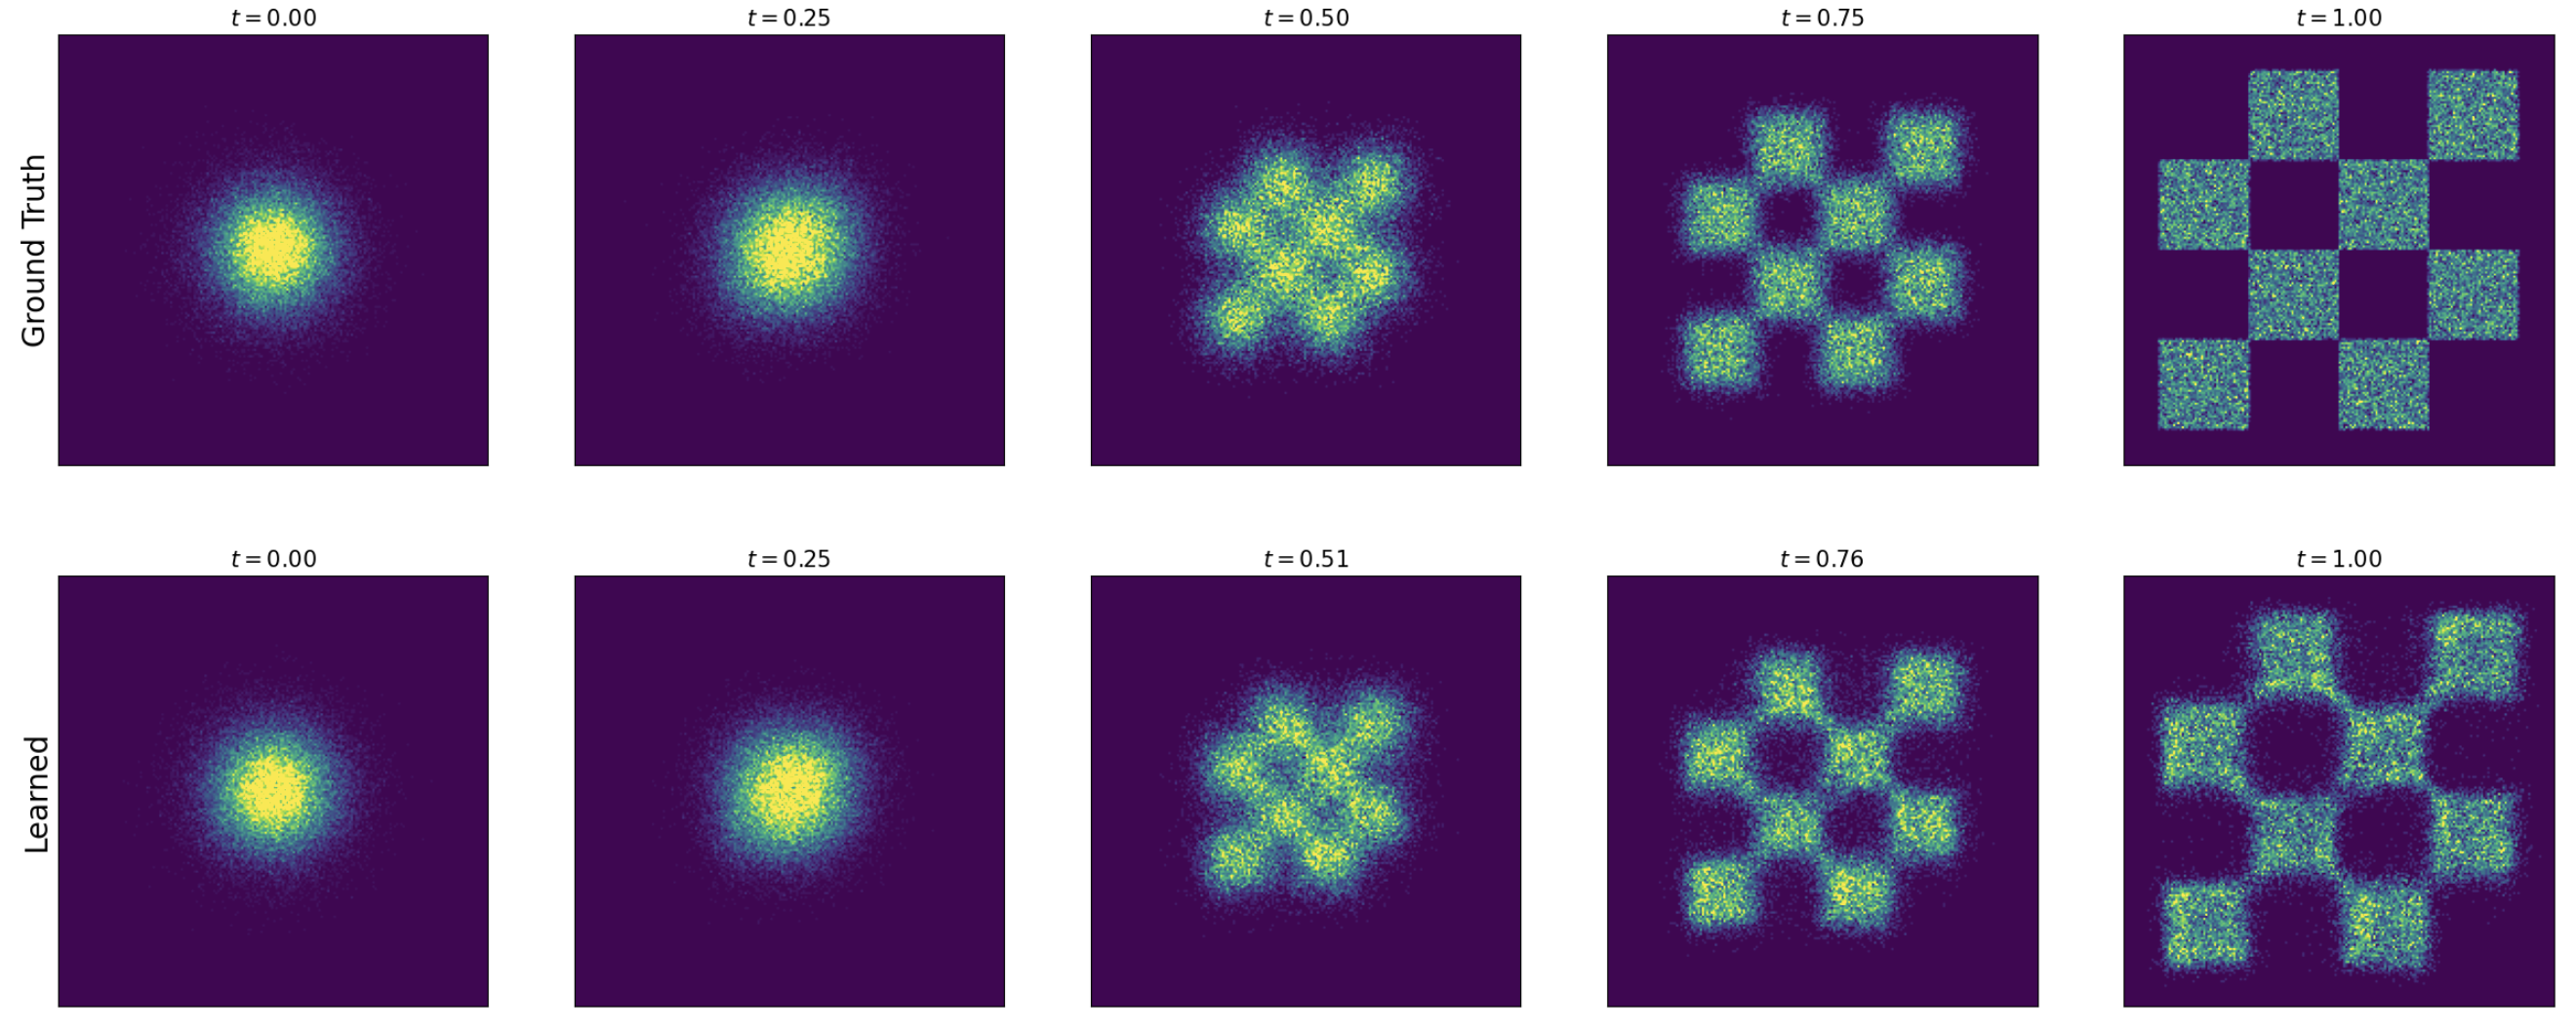
\includegraphics[width=\textwidth]{figures/conditional_marginal_path.png} &
         % \includegraphics[width=0.22\textwidth]{assets/flow_velocity/flow_v_5.png} &
         % 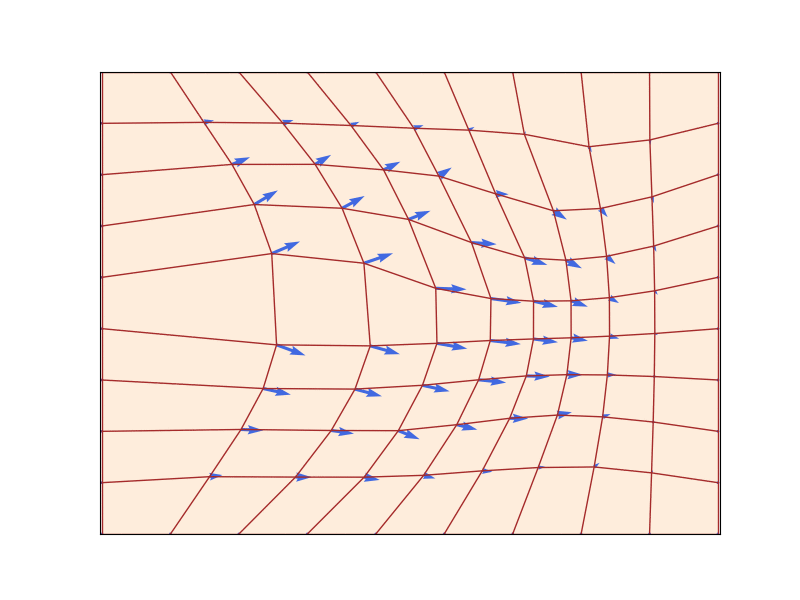
\includegraphics[width=0.3\textwidth]{fm_guide_assets/flow_10.png} &
         % % \includegraphics[width=0.22\textwidth]{assets/flow_velocity/flow_v_14.png} &
         % 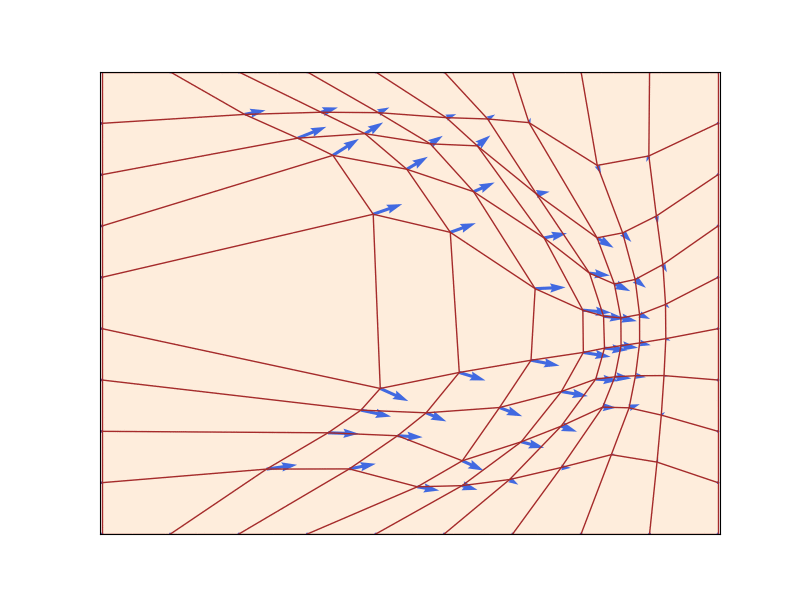
\includegraphics[width=0.3\textwidth]{fm_guide_assets/flow_16.png} 
    \end{tabular}
    \caption{\label{fig:fm_illustration_checkerboard}Illustration of \cref{thm:fm_loss} with a Gaussian CondOT probability path: simulating an ODE from a trained flow matching model. The data distribution is the chess board pattern (top right). Top row: Histogram from ground truth marginal probability path $p_t(x)$. Bottom row: Histogram of samples from flow matching model. As one can see, the top row and bottom row match after training (up to training error). The model was trained using \cref{alg:training_fm_score_matching_gaussian_paths}.}

使用高斯 CondOT 概率路径对\cref{thm:fm_loss}的说明:从训练好的流匹配模型模拟 ODE。数据分布是棋盘图案(右上)。上行:来自真实边际概率路径 $p_t(x)$ 的直方图。下行:来自流匹配模型样本的直方图。可以看出,训练后上行和下行匹配(除了训练误差)。该模型使用\cref{alg:training_fm_score_matching_gaussian_paths}进行训练。
\end{figure}

% When I first saw \cref{thm:fm_loss}, I found it a big magical: Without seeing $\uref_t(x)$ explicitly ever, we can approximate it implicitly with a neural network. Therefore, \cref{thm:fm_loss} gives us a powerful of training our ODE generative model by minimizing $\Lcond(\theta)$. All we have to do is minimize a simple mean squared error. This is scalable to very large datasets in high dimensions and can be implemented in a few lines of code. When tracking the training, you should keep in mind that \textbf{the absolute value of the loss is meaningless} (you will never achieve zero loss because $C<0$). This makes it sometimes a little tricky to realize when the training is converged.
\subsection{Score Matching}

Let us extend the algorithm we just found from ODEs to SDEs. Remember we can extend the target ODE to an SDE with the same marginal distribution given by
\begin{align}
\label{eq:sde_extension_restated}
    \dd X_t &=\left[\uref_t(X_t)+\frac{\sigma_t^2}{2}\nabla\log p_t(X_t)\right]\dd t +\sigma_t\dd W_t\\
    X_0&\sim\pinit,\quad \\
    \label{eq:marginal_ode_follows_marginal_path_restated}
    \Rightarrow X_t&\sim p_t\quad (0\leq t\leq 1)
\end{align}
where $\uref_t$ is the marginal vector field and $\nabla\log p_t(x)$ is the \themebf{marginal score} function represented via the formula
\begin{align}
\label{eq:score_marginal_restated}
\nabla\log p_t(x) =&\int \nabla \log p_t(x|z)\frac{ p_t(x|z)\pdata(z)}{p_t(x)}\,\dd z.
\end{align}
To approximate the marginal score $\nabla\log p_t$, we can use a neural network that we call \themebf{score network} $s_t^\theta:\mathbb{R}^d\times[0,1]\to\mathbb{R}^d$. In the same way as before, we can design a \themebf{score matching} loss and a \themebf{conditional score matching} loss:

让我们将刚刚找到的算法从 ODE 扩展到 SDE。回忆我们可以将目标 ODE 扩展为具有相同边际分布的 SDE,由下式给出:
\begin{align}
\label{eq:sde_extension_restated}
    \dd X_t &=\left[\uref_t(X_t)+\frac{\sigma_t^2}{2}\nabla\log p_t(X_t)\right]\dd t +\sigma_t\dd W_t\\
    X_0&\sim\pinit,\quad \\
    \label{eq:marginal_ode_follows_marginal_path_restated}
    \Rightarrow X_t&\sim p_t\quad (0\leq t\leq 1)
\end{align}
其中 $\uref_t$ 是边际向量场,$\nabla\log p_t(x)$ 是通过以下公式表示的\themebf{边际分数}函数:
\begin{align}
\label{eq:score_marginal_restated}
\nabla\log p_t(x) =&\int \nabla \log p_t(x|z)\frac{ p_t(x|z)\pdata(z)}{p_t(x)}\,\dd z.
\end{align}
为了近似边际分数 $\nabla\log p_t$,我们可以使用一个神经网络,我们称之为\themebf{分数网络} $s_t^\theta:\mathbb{R}^d\times[0,1]\to\mathbb{R}^d$。与之前相同的方式,我们可以设计一个\themebf{分数匹配}损失和一个\themebf{条件分数匹配}损失:
\begin{align}
    \mathcal{L}_{\text{SM}}(\theta) &=\mathbb{E}_{t\sim\text{Unif},z\sim \pdata, x\sim p_t(\cdot|\dap)}[\|s_t^\theta(x) - \nabla\log p_t(x)\|^2] &&\blacktriangleright\,\,\text{score matching loss/分数匹配损失}\nonumber\\
    \mathcal{L}_{\text{CSM}}(\theta) &=\mathbb{E}_{t\sim\text{Unif},z\sim \pdata, x\sim p_t(\cdot|\dap)}[\|s_t^\theta(x) - \nabla\log p_t(x|\dap)\|^2]  &&\blacktriangleright\,\,\text{conditional score matching loss/条件分数匹配损失}\label{eq:dsm}
\end{align}
where again the difference is using the marginal score $\nabla\log p_t(x)$ vs. using the conditional score $\nabla\log p_t(x|z)$. %\footnote{It would be more consistent to call it \emph{conditional} score matching loss but \emph{denoising} score matching is a term used in the literature. We will realize later why it is called \emph{denoising} score matching.} 
As before, we ideally would want to minimize the score matching loss but can't because we don't know $\nabla\log p_t(x)$. But similarly as before, the conditional score matching loss is a tractable alternative:

其中区别再次是使用边际分数 $\nabla\log p_t(x)$ 与使用条件分数 $\nabla\log p_t(x|z)$。如前所述,我们理想情况下希望最小化分数匹配损失,但由于我们不知道 $\nabla\log p_t(x)$,所以无法做到。但与之前类似,条件分数匹配损失是一个可处理的替代方案:
\begin{theorem}
\label{thm:dsm_loss}
The score matching loss equals the conditional score matching loss up to a constant:

得分匹配损失等于条件得分匹配损失加上一个常数:

\begin{align*}
\mathcal{L}_{\text{SM}}(\theta) = \mathcal{L}_{\text{CSM}}(\theta) + C,
\end{align*}

where $C$ is independent of parameters $\theta$. Therefore, their gradients coincide:

其中 $C$ 与参数 $\theta$ 无关。因此,它们的梯度重合:

\begin{align*}
\nabla_\theta \mathcal{L}_{\text{SM}}(\theta) = \nabla_\theta \mathcal{L}_{\text{CSM}}(\theta).
\end{align*}

In particular, for the minimizer $\theta^*$, it will hold that $s_t^{\theta^*}=\nabla\log p_t$. 

特别地,对于最小化器 $\theta^*$,将有 $s_t^{\theta^*}=\nabla\log p_t$。
\end{theorem}
\begin{proof}
Note that the formula for $\nabla\log p_t$ (\cref{eq:score_marginal_restated}) looks the same as the formula for $\uref_t$ (\cref{eq:marginal_vector_field_stated_again}). Therefore, the proof is identical to the proof of \cref{thm:fm_loss} replacing $\uref_t$ with $\nabla\log p_t$.

注意 $\nabla\log p_t$ 的公式(\cref{eq:score_marginal_restated})与 $\uref_t$ 的公式(\cref{eq:marginal_vector_field_stated_again})看起来相同。因此,证明与 \cref{thm:fm_loss} 的证明相同,只需将 $\uref_t$ 替换为 $\nabla\log p_t$。
\end{proof}

The above procedure describes the vanilla procedure of training a diffusion model. After training, we can choose an arbitrary diffusion coefficient $\sigma_t\geq 0$ and then simulate the SDE

上述过程描述了训练扩散模型的标准过程。训练后,我们可以选择任意扩散系数 $\sigma_t\geq 0$,然后模拟 SDE
\begin{align}
\label{eq:sde_extension_restated}
    X_0\sim&\pinit,\quad \dd X_t =\left[u_t^\theta(X_t)+\frac{\sigma_t^2}{2}s_t^\theta(X_t)\right]\dd t +\sigma_t\dd W_t,
\end{align}
to generate samples $X_1\sim\pdata$. In theory, every $\sigma_t$ should give samples $X_1\sim \pdata$ at perfect training. In practice, we encounter two types of errors: (1) numerical errors by simulating the SDE imperfectly and (2) training errors (i.e., the model $u_t^{\theta}$ is not exactly equal to $\uref_t$). Therefore, there is an optimal unknown noise level $\sigma_t$ - this can be determined empirically by just testing our different values of empirically (see e.g. \citep{albergo2023stochastic,karras2022elucidating,ma2024sit}).

生成样本 $X_1\sim\pdata$。理论上,在完美训练的情况下,每个 $\sigma_t$ 都应该生成样本 $X_1\sim \pdata$。实际上,我们会遇到两种类型的误差:(1)通过不完美地模拟 SDE 产生的数值误差,以及(2)训练误差(即模型 $u_t^{\theta}$ 不完全等于 $\uref_t$)。因此,存在一个最优的未知噪声水平 $\sigma_t$ - 这可以通过经验性地测试我们的不同值来确定(例如参见 \citep{albergo2023stochastic,karras2022elucidating,ma2024sit})。

At first sight, it might seem to be a disadvantage that we have to learn both $s_t^\theta$ and $u_t^\theta$ if we wanted to use diffusion model now as opposed to a flow model. However, note we can often directly $s_t^\theta$ and $u_t^\theta$ in a single network with two outputs, so that the additional computational effort is usually minimal. Further, as we will see now for the special case of the Gaussian probability path, $s_t^\theta$ and $u_t^\theta$ may be converted into one another so that we don't have to train them separately.

乍一看,如果我们现在想要使用扩散模型而不是流模型,我们必须同时学习 $s_t^\theta$ 和 $u_t^\theta$ 似乎是一个缺点。然而,注意我们通常可以在一个具有两个输出的单一网络中直接学习 $s_t^\theta$ 和 $u_t^\theta$,因此额外的计算工作量通常是最小的。此外,正如我们现在将看到的,对于高斯概率路径的特殊情况,$s_t^\theta$ 和 $u_t^\theta$ 可以相互转换,因此我们不必单独训练它们。

\begin{remarkbox}[Denoising Diffusion Models]If you are familiar with diffusion models, you have probably encountered the term \themebf{\textit{denoising} diffusion model}. This model has become so popular that most people nowadays drop the word "denoising" and simply use the term "diffusion model" to describe it. In the language of this document, these are simply diffusion models with Gaussian probability paths $p_t(\cdot|z)=\mathcal{N}(\alpha_t z;\beta_t^2 I_d)$.

如果你熟悉扩散模型,你可能遇到过\themebf{\textit{去噪}扩散模型}这个术语。这种模型已经变得如此流行,以至于现在大多数人都省略了"去噪"一词,而简单地使用"扩散模型"来描述它。在本文档的语言中,这些只是具有高斯概率路径 $p_t(\cdot|z)=\mathcal{N}(\alpha_t z;\beta_t^2 I_d)$ 的扩散模型。

However, it is important to note that this might not be immediately obvious if you read some of the first diffusion model papers: they use a different time convention (time is inverted) - so you need apply an appropriate time re-scaling - and they construct their probability path via so-called \textbf{forward processes} (we will discuss this in \cref{subsec:guide_to_flow_matching_literature}).

然而,需要注意的是,如果你阅读一些早期的扩散模型论文,这一点可能不会立即显而易见:它们使用不同的时间约定(时间是反转的)- 因此你需要应用适当的时间重新缩放 - 并且它们通过所谓的\textbf{前向过程}来构建概率路径(我们将在\cref{subsec:guide_to_flow_matching_literature}中讨论这一点)。
\end{remarkbox}

\begin{examplebox}[Denoising Diffusion Models: Score Matching for Gaussian Probability Paths]
First, let us instantiate the denoising score matching loss for the case of $p_t(x|z)=\mathcal{N}(\alpha_tz,\beta_t^2I_d)$. As we derived in \cref{eq:cond_score_gaussian}, the conditional score $\nabla\log p_t(x|z)$ has the formula
\begin{align}
\label{e:marginal_vf_cond_score_restated}
    \nabla\log p_t(x|z) = -\frac{x-\alpha_t z}{\beta_t^2}.
\end{align}
Plugging in this formula, the conditional score matching loss becomes:
\begin{align*}
        \mathcal{L}_{\text{CSM}}(\theta) &=\mathbb{E}_{t\sim\Unif,z\sim \pdata, x\sim p_t(\cdot|\dap)}[\|s_t^\theta(x)+\frac{x-\alpha_t z}{\beta_t^2}\|^2]\\&\overset{(i)}{=}\mathbb{E}_{t\sim\Unif,z\sim \pdata, \epsilon\sim \mathcal{N}(0,I_d)}[\|s_t^\theta(\alpha_tz+\beta_t\epsilon)+\frac{\epsilon}{\beta_t}\|^2]\\
        &=\mathbb{E}_{t\sim\Unif,z\sim \pdata, \epsilon\sim \mathcal{N}(0,I_d)}[\frac{1}{\beta_t^2}\|\beta_ts_t^\theta(\alpha_tz+\beta_t\epsilon)+\epsilon\|^2]
\end{align*}
where in $(i)$ we plugged in \cref{eq:sampling_procedure_gaussian_path_restated_for_fm} and replaced $x$ by $\alpha_tz+\beta_t\epsilon$. Note that the network $s_t^\theta$ essentially learns to predict the noise that was used to corrupt a data sample $z$. Therefore, the above training loss is also called \themebf{denoising score matching} and it was the one of the first procedures used to learn diffusion models. It was soon realized that the above loss is numerically unstable for $\beta_t\approx 0$ close to zero (i.e. denoising score matching only works if you add a sufficient amount of noise). In some of the first works on denoising diffusion models (see \textbf{Denoising Diffusion Probabilitic Models}, \citep{ho2020denoising}) it was therefore proprosed to drop the constant $\frac{1}{\beta_t^2}$ in the loss and reparameterize $s_t^\theta$ into a \themebf{noise predictor} network $\epsilon_t^\theta:\mathbb{R}^d\times[0,1]\to\mathbb{R}^d$ via:
\begin{align*}
    -\beta_t s_t^\theta(x) = \epsilon_t^\theta(x)\quad \Rightarrow \quad \mathcal{L}_{\text{DDPM}}(\theta) =&\mathbb{E}_{t\sim\Unif,z\sim \pdata, \epsilon\sim \mathcal{N}(0,I_d)}\left[\|\epsilon_t^\theta(\alpha_tz+\beta_t\epsilon)-\epsilon\|^2\right]
\end{align*}
As before, the network $\epsilon_t^\theta$ essentially learns to predict the noise that was used to corrupt a data sample $z$. In \cref{alg:training_score_matching_gaussian_paths}, we summarize the training procedure.

首先,让我们为 $p_t(x|z)=\mathcal{N}(\alpha_tz,\beta_t^2I_d)$ 的情况实例化去噪分数匹配损失。正如我们在\cref{eq:cond_score_gaussian}中推导的,条件分数 $\nabla\log p_t(x|z)$ 的公式为:
\begin{align}
\label{e:marginal_vf_cond_score_restated}
    \nabla\log p_t(x|z) = -\frac{x-\alpha_t z}{\beta_t^2}.
\end{align}
将此公式代入,条件分数匹配损失变为:
\begin{align*}
        \mathcal{L}_{\text{CSM}}(\theta) &=\mathbb{E}_{t\sim\Unif,z\sim \pdata, x\sim p_t(\cdot|\dap)}[\|s_t^\theta(x)+\frac{x-\alpha_t z}{\beta_t^2}\|^2]\\&\overset{(i)}{=}\mathbb{E}_{t\sim\Unif,z\sim \pdata, \epsilon\sim \mathcal{N}(0,I_d)}[\|s_t^\theta(\alpha_tz+\beta_t\epsilon)+\frac{\epsilon}{\beta_t}\|^2]\\
        &=\mathbb{E}_{t\sim\Unif,z\sim \pdata, \epsilon\sim \mathcal{N}(0,I_d)}[\frac{1}{\beta_t^2}\|\beta_ts_t^\theta(\alpha_tz+\beta_t\epsilon)+\epsilon\|^2]
\end{align*}
其中在 $(i)$ 中我们代入了\cref{eq:sampling_procedure_gaussian_path_restated_for_fm}并用 $\alpha_tz+\beta_t\epsilon$ 替换了 $x$。注意网络 $s_t^\theta$ 本质上学习预测用于破坏数据样本 $z$ 的噪声。因此,上述训练损失也被称为\themebf{去噪分数匹配},它是用于学习扩散模型的最早程序之一。很快人们意识到,对于接近零的 $\beta_t\approx 0$,上述损失在数值上是不稳定的(即去噪分数匹配只有在添加足够噪声时才有效)。在一些关于去噪扩散模型的早期工作中(参见\textbf{去噪扩散概率模型},\citep{ho2020denoising}),因此提出在损失中去掉常数 $\frac{1}{\beta_t^2}$,并将 $s_t^\theta$ 重新参数化为\themebf{噪声预测器}网络 $\epsilon_t^\theta:\mathbb{R}^d\times[0,1]\to\mathbb{R}^d$:
\begin{align*}
    -\beta_t s_t^\theta(x) = \epsilon_t^\theta(x)\quad \Rightarrow \quad \mathcal{L}_{\text{DDPM}}(\theta) =&\mathbb{E}_{t\sim\Unif,z\sim \pdata, \epsilon\sim \mathcal{N}(0,I_d)}\left[\|\epsilon_t^\theta(\alpha_tz+\beta_t\epsilon)-\epsilon\|^2\right]
\end{align*}
如前所述,网络 $\epsilon_t^\theta$ 本质上学习预测用于破坏数据样本 $z$ 的噪声。在\cref{alg:training_score_matching_gaussian_paths}中,我们总结了训练过程。
\end{examplebox}

\begin{algorithm}[h]
\caption{Score Matching Training Procedure for Gaussian probability path / 高斯概率路径的分数匹配训练过程}
\label{alg:training_score_matching_gaussian_paths}
\begin{algorithmic}[1]
\REQUIRE A dataset of samples $z\sim \pdata$, score network $s_t^\theta$ or noise predictor $\epsilon_t^\theta$ / 样本数据集 $z\sim \pdata$,分数网络 $s_t^\theta$ 或噪声预测器 $\epsilon_t^\theta$
\FOR{each mini-batch of data / 对于每个数据小批量}
    \STATE Sample a data example $\dap$ from the dataset. / 从数据集中采样一个数据示例 $\dap$。
    \STATE Sample a random time $t \sim \text{Unif}_{[0,1]}$. / 采样一个随机时间 $t \sim \text{Unif}_{[0,1]}$。
    \STATE Sample noise $\epsilon\sim\mathcal{N}(0,I_d)$ / 采样噪声 $\epsilon\sim\mathcal{N}(0,I_d)$
    \STATE Set $x_t=\alpha_t z + \beta_t\epsilon$\hfill (\text{General case: }$x_t\sim p_t(\cdot|z)$) / 设置 $x_t=\alpha_t z + \beta_t\epsilon$\hfill (\text{一般情况: }$x_t\sim p_t(\cdot|z)$)
    %\IF{Flow matching}
    \STATE Compute loss / 计算损失
    \begin{align*}
        \mathcal{L}(\theta) =& \|s_t^\theta(x_t)+\frac{\epsilon}{\beta_t}\|^2 \quad &(\text{General case: }=\|s_t^\theta(x_t)-\nabla\log p_t(x_t|z)\|^2)\\
    \text{Alternatively: }\mathcal{L}(\theta) =& \|\epsilon_t^\theta(x_t)-\epsilon\|^2
    \end{align*}
    %\ENDIF
    % \IF{Score matching}
    % \STATE
    % \begin{align*}
    %     \mathcal{L}(\theta) =& \|s_t^\theta(x_t)+\frac{\epsilon}{\beta_t}\|^2 \quad &(\text{General case: }=\|s_t^\theta(x_t)+\nabla\log p_t(x_t|z)\|^2)
    % \end{align*}
    % \ENDIF
    \STATE Update the model parameters $\theta$ via gradient descent on $\mathcal{L}(\theta)$. / 通过对 $\mathcal{L}(\theta)$ 进行梯度下降来更新模型参数 $\theta$。
\ENDFOR
\end{algorithmic}
\end{algorithm}
Beyond its simplicity, there is another useful property of the Gaussian probability path: By learning $s_t^\theta$ or $\epsilon_t^\theta$, we also learn $u_t^\theta$ automatically and the other way around: / 除了简单性之外,高斯概率路径还有另一个有用的性质:通过学习 $s_t^\theta$ 或 $\epsilon_t^\theta$,我们也自动学习了 $u_t^\theta$,反之亦然:

除了其简单性之外,高斯概率路径还有另一个有用的性质:通过学习 $s_t^\theta$ 或 $\epsilon_t^\theta$,我们也自动学习了 $u_t^\theta$,反之亦然:
\begin{proposition}[Conversion formula for Gaussian probability path]
\label{prop:conversion_formula_gaussian_prob_path}
For the Gaussian probability path $p_t(x|z)=\mathcal{N}(\alpha_t z,\beta_t^2 I_d)$, it holds that that the conditional (resp. marginal) vector field can be converted into the conditional (resp. marginal) score:

对于高斯概率路径 $p_t(x|z)=\mathcal{N}(\alpha_t z,\beta_t^2 I_d)$,条件(相应地,边际)向量场可以转换为条件(相应地,边际)分数:
\begin{align*}
\uref_t(x|z)=\left(\beta_t^2\frac{\dot{\alpha}_t}{\alpha_t}-\dot{\beta}_t\beta_t\right)\nabla\log p_t(x|z)+\frac{\dot{\alpha}_t}{\alpha_t}x\\
\uref_t(x)=\left(\beta_t^2\frac{\dot{\alpha}_t}{\alpha_t}-\dot{\beta}_t\beta_t\right)\nabla\log p_t(x)+\frac{\dot{\alpha}_t}{\alpha_t}x
\end{align*}
where the formula for the above marginal vector field $\uref_t$ is called \themebf{probability flow ODE} in the literature (more correctly, the corresponding ODE).

其中上述边际向量场 $\uref_t$ 的公式在文献中被称为\themebf{概率流ODE}(更准确地说,是相应的ODE)。
\end{proposition}
\begin{proof}
For the conditional vector field and conditional score, we can derive:

对于条件向量场和条件分数,我们可以推导:
\begin{align*}
\uref_t(x|z)=&\left(\dot{\alpha}_t-\frac{\dot{\beta}_t}{\beta_t}\alpha_t\right)z+\frac{\dot{\beta}_t}{\beta_t}x
\overset{(i)}{=}\left(\beta_t^2\frac{\dot{\alpha}_t}{\alpha_t}-\dot{\beta}_t\beta_t\right)\left(\frac{\alpha_tz-x}{\beta_t^2}\right)+\frac{\dot{\alpha}_t}{\alpha_t}x=\left(\beta_t^2\frac{\dot{\alpha}_t}{\alpha_t}-\dot{\beta}_t\beta_t\right)\nabla\log p_t(x|z)+\frac{\dot{\alpha}_t}{\alpha_t}x
\end{align*}
where in $(i)$ we just did some algebra. By taking integrals, the same identity holds for the marginal flow vector field and the marginal score function:

其中在$(i)$中我们只是做了一些代数运算。通过积分,相同的恒等式适用于边际流向量场和边际分数函数:
\begin{align*}
\uref(x)= \int \uref_t(x|z)\frac{ p_t(x|z)\pdata(z)}{p_t(x)}\dd z
=&\int\left[\left(\beta_t^2\frac{\dot{\alpha}_t}{\alpha_t}-\dot{\beta}_t\beta_t\right)\nabla\log p_t(x|z)+\frac{\dot{\alpha}_t}{\alpha_t}x\right] \frac{ p_t(x|z)\pdata(z)}{p_t(x)}\dd z\\
\overset{(i)}{=}&\left(\beta_t^2\frac{\dot{\alpha}_t}{\alpha_t}-\dot{\beta}_t\beta_t\right)\nabla\log p_t(x)+\frac{\dot{\alpha}_t}{\alpha_t}x
\end{align*}
where in $(i)$ we used \cref{eq:score_marginal_restated}.

其中在$(i)$中我们使用了\cref{eq:score_marginal_restated}。
\end{proof}
\begin{figure}[!h]
    \centering
    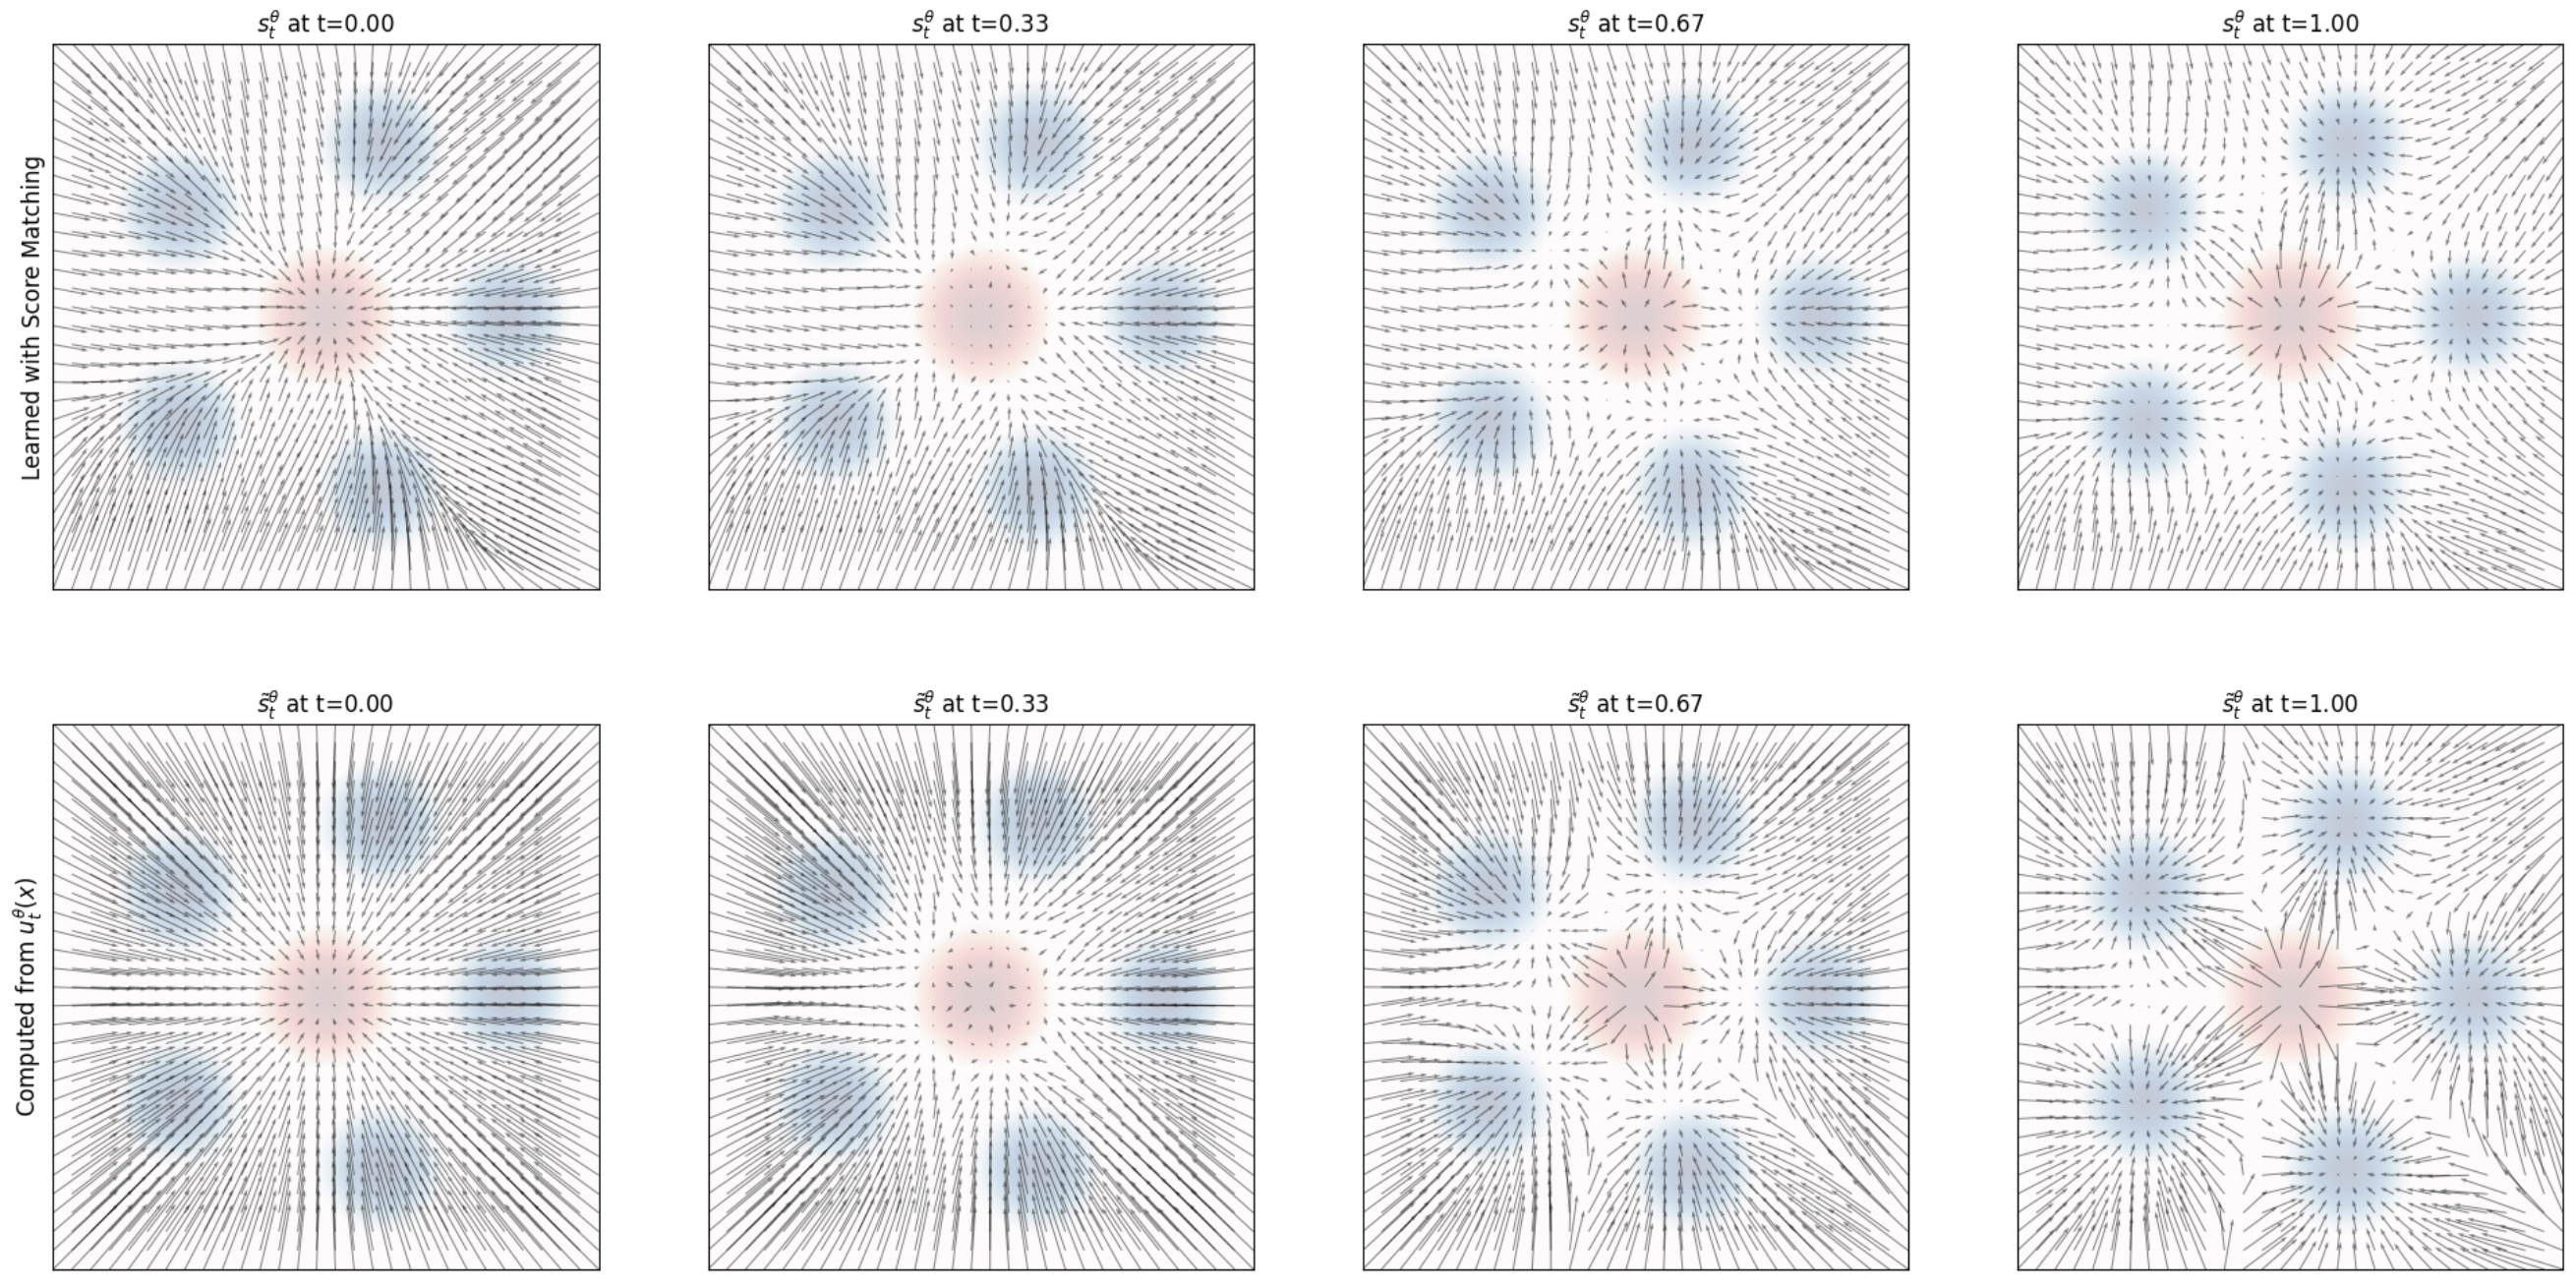
\includegraphics[width=\linewidth]{figures/score_field_comparison.png}
    \caption{\label{fig:score_fields}A comparison of the score, as obtained in two different ways. Top: A visualization of the score field $s_t^\theta(x)$ learned independently with score matching (see \cref{alg:training_score_matching_gaussian_paths}). Bottom: A visualization of the score field $\tilde{s}_t^\theta(x)$ parameterized using $u_t^\theta(x)$ as in \cref{eq:marginal_vf_to_score_formula}.}
    
    两种不同方式获得的分数的比较。顶部:独立使用分数匹配学习的分数场 $s_t^\theta(x)$ 的可视化(见\cref{alg:training_score_matching_gaussian_paths})。底部:使用 $u_t^\theta(x)$ 参数化的分数场 $\tilde{s}_t^\theta(x)$ 的可视化,如\cref{eq:marginal_vf_to_score_formula}所示。
\end{figure}
We can use the conversion formula to parameterize the score network $s_t^\theta$ and the vector field network $u_t^\theta$ into one another via 
\begin{align}
u_t^\theta=\left(\beta_t^2\frac{\dot{\alpha}_t}{\alpha_t}-\dot{\beta}_t\beta_t\right)s_t^\theta(x)+\frac{\dot{\alpha}_t}{\alpha_t}x.
\label{eq:marginal_score_to_vf_formula}
\end{align}
Similarly, so long as $\beta_t^2\dot{\alpha}_t -\alpha_t\dot{\beta}_t\beta_t \neq 0$ (always true for $t \in [0,1)$), it follows that

类似地,只要 $\beta_t^2\dot{\alpha}_t -\alpha_t\dot{\beta}_t\beta_t \neq 0$(对于 $t \in [0,1)$ 总是成立),那么
\begin{align}
s_t^\theta(x) = \frac{\alpha_t u_t^\theta(x) - \dot{\alpha}_tx}{\beta_t^2\dot{\alpha}_t -\alpha_t\dot{\beta}_t\beta_t}.
\label{eq:marginal_vf_to_score_formula}
\end{align}
Using this parameterization, it can be shown that the denoising score matching and the conditional flow matching losses are the same up to a constant. We conclude that \textbf{for Gaussian probability paths there is no need to separately train both the marginal score and the marginal vector field, as knowledge of one is sufficient to compute the other. In particular, we can choose whether we want to use flow matching or score matching to train it}. In \cref{fig:score_fields}, we compare visually the score as approximated using score matching and the parameterized score using \cref{eq:marginal_vf_to_score_formula}. If we have trained a score network $s_t^\theta$, we know by \cref{eq:sde_extension_restated} that we can use arbitrary $\sigma_t\geq 0$ to sample from the SDE

使用这种参数化,可以证明去噪分数匹配和条件流匹配损失在常数范围内是相同的。我们得出结论:\textbf{对于高斯概率路径,没有必要分别训练边际分数和边际向量场,因为其中一个的知识足以计算另一个。特别地,我们可以选择是使用流匹配还是分数匹配来训练它}。在\cref{fig:score_fields}中,我们直观地比较了使用分数匹配近似的分数和使用\cref{eq:marginal_vf_to_score_formula}参数化的分数。如果我们训练了一个分数网络 $s_t^\theta$,我们通过\cref{eq:sde_extension_restated}知道我们可以使用任意的 $\sigma_t\geq 0$ 从SDE中采样
\begin{align}
    X_0\sim&\pinit,\quad \dd X_t =\left[\left(\beta_t^2\frac{\dot{\alpha}_t}{\alpha_t}-\dot{\beta}_t\beta_t+\frac{\sigma_t^2}{2}\right)s_t^\theta(x)+\frac{\dot{\alpha}_t}{\alpha_t}x\right]\dd t +\sigma_t\dd W_t
\end{align}
to obtain samples $X_1\sim \pdata$ (up to training and simulation error). This corresponds to \themebf{stochastic sampling from a denoising diffusion model.}

以获得样本 $X_1\sim \pdata$(直到训练和仿真误差)。这对应于\themebf{从去噪扩散模型的随机采样。}


% \subsection{Primer: How to learn conditional expectations}
% We start off by a reminder about some fundamental statistics. Specifically, we briefly discuss on how to approximate (conditional) expectations of some random variables by using the mean squared error.

% \paragraph{Learning an average.} Let us assume that $Z\in\mathbb{R}^k$ is a random variable. Imagine that we want to find the vector $\mathbb{E}[Z]\in\mathbb{R}^k$ given the expected value of $Z$. We can frame this as the following minimization problem of the \themebf{mean squared error}:
% \begin{align}
% \label{eq:average_as_minimization}
%     \mathbb{E}_{Z}[Z] = \argmin\limits_{v\in\mathbb{R}^k}\mathbb{E}_{Z}[\|Z-v\|^2]
% \end{align}
% In other words, the best constant guess $v$ of $Z$ as measured by the mean-squared error is the expected value of $Z$. To see that the above holds, one can do the following calculation for an arbitrary $v$
% \begin{align*}
%     \mathbb{E}[\|Z-v\|^2] =& \mathbb{E}[\|(Z-\mathbb{E}[Z])+(\mathbb{E}[Z]-v)\|^2]\\
% \overset{(i)}{=}&\mathbb{E}[\|Z-\mathbb{E}[Z]\|^2+2(Z-\mathbb{E}[Z])^T(\mathbb{E}[Z]-v)]+\|\mathbb{E}[Z]-v\|^2\\
% \overset{(ii)}{=}&\mathbb{E}[\|Z-\mathbb{E}[Z]\|^2]+2(\mathbb{E}[Z]-\mathbb{E}[Z])^T(\mathbb{E}[Z]-v)+\|\mathbb{E}[Z]-v\|^2\\
% =&\mathbb{E}[\|Z-\mathbb{E}[Z]\|^2]+\|\mathbb{E}[Z]-v)\|^2\\
% \geq & \mathbb{E}[\|Z-\mathbb{E}[Z]\|^2]
% \end{align*}
% where in $(i)$ we used that identity $\|a+b\|^2=\|a\|^2+2a^Tb+\|b\|^2$ and $(ii)$ we used the fact that the expected value is linear. The last inequality becomes an equality if and only if $v=\mathbb{E}[Z]$. This proves \cref{eq:average_as_minimization}.


% \paragraph{Learning a conditional average.} Let us now imagine that we have two random variables $X\in\mathbb{R}^d,Z\in\mathbb{R}^k$ jointly sampled (i.e. they might be coupled). Let us imagine that we know that $X=x$ and we want to estimate $Z$. Naturally, in machine learning we would choose a parameterized function $F^\theta:\mathbb{R}^d\to\mathbb{R}^k$ (usually $F^\theta$ is a neural network) and then minimize the mean square error
% \begin{align*}
%     L(\theta) =& \mathbb{E}_{X,Z}[\|F^\theta(X)-Z\|^2]
% \end{align*}
% We can 
% \begin{align*}
%     L(\theta) =& \mathbb{E}_{X}[\mathbb{E}[\|F^\theta(X)-Z\|^2|X]]
% \end{align*}
% The best estimate is given by the \themebf{conditional expectation} 
% \begin{align*}
%     F^{\theta^*} = \mathbb{E}[Z|X=x]
% \end{align*}
% Note that the conditional expectation is a function of $x$. How would we approximate it?
% Therefore, we learnt: \textbf{training a neural network by minimizing a mean squared error results in the neural network approximating the conditional expectation.}

\subsection{A Guide to the  Diffusion Model Literature}
\label{subsec:guide_to_flow_matching_literature}

There is a whole family of models around diffusion models and flow matching in the literature. When you read these papers, you will likely find a different (but equivalent) way of presenting the material from this class. This makes it sometimes a little confusing to read these papers. For this reason, we want to give a brief overview over various frameworks and their differences and put them also in their historical context. \textbf{This is not necessary to understand the remainder of this document} but rather intended to be a support for you in case you read the literature.

文献中存在围绕扩散模型和流匹配的整个模型族。当你阅读这些论文时,你可能会发现与本课程不同(但等价)的材料呈现方式。这有时会让阅读这些论文感到有些困惑。因此,我们想要简要概述各种框架及其差异,并将它们放在历史背景中。\textbf{这对于理解本文档的其余部分不是必需的},而是在你阅读文献时为你提供支持。

\paragraph{Discrete time vs. continuous time.} The first denoising diffusion model papers \citep{sohl2015deep, song2019generative, ho2020denoising} did not use SDEs but constructed Markov chains in \themebf{discrete time}, i.e. with time steps $t=0,1,2,3,\dots$. To this date, you will find a lot of works in the literature working with this discrete-time formulation. While this construction is appealing due to its simplicity, the disadvantage of the time-discrete approach is that it forces you to choose a time discretization before training. Further, the loss function needs to be approximated via an \themebf{evidence lower bound (ELBO)} - which is, as the name suggests, only a lower bound to the loss we actually want to minimize. Later, \citet{song2020score} showed that these constructions were essentially an approximation of a time-continuous SDEs. Further, the ELBO loss becomes tight (i.e. it is not a lower bound anymore) in the continuous time case (e.g. note that \cref{thm:fm_loss} and \cref{thm:dsm_loss} are equalities and not lower bounds - this would be different in the discrete time case). This made the SDE construction popular because it was considered mathematically "cleaner" and that one could control the simulation error via ODE/SDE samplers post training. It is important to note however that both models employ the same loss and are \textit{not} fundamentally different.

第一批去噪扩散模型论文\citep{sohl2015deep, song2019generative, ho2020denoising}没有使用SDE,而是在\themebf{离散时间}中构造马尔可夫链,即时间步长为 $t=0,1,2,3,\dots$。至今,你会在文献中发现很多使用这种离散时间表述的工作。虽然这种构造由于其简单性而很有吸引力,但时间离散方法的缺点是它强迫你在训练前选择时间离散化。此外,损失函数需要通过\themebf{证据下界(ELBO)}来近似——顾名思义,这只是我们实际想要最小化的损失的下界。后来,\citet{song2020score}表明这些构造本质上是时间连续SDE的近似。此外,ELBO损失在连续时间情况下变得紧致(即不再是下界)(例如,注意\cref{thm:fm_loss}和\cref{thm:dsm_loss}是等式而不是下界——这在离散时间情况下会有所不同)。这使得SDE构造变得流行,因为它被认为在数学上更"干净",并且可以在训练后通过ODE/SDE采样器控制仿真误差。然而,重要的是要注意两种模型使用相同的损失,并且在根本上\textit{没有}不同。

\paragraph{"Forward process" vs probability paths.} The first wave of denoising diffusion models \citep{sohl2015deep, song2019generative, ho2020denoising, song2020score} did not use the term \themebf{probability path} but constructed a noising procedure of a data point $z\in\mathbb{R}^d$ via a so-called \themebf{forward process}. This is an SDE of the form

第一波去噪扩散模型\citep{sohl2015deep, song2019generative, ho2020denoising, song2020score}没有使用\themebf{概率路径}这个术语,而是通过所谓的\themebf{前向过程}构造了数据点 $z\in\mathbb{R}^d$ 的噪声程序。这是一个形式为:
\begin{align}
\label{eq:forward_process}
    \bar{X}_0=z,\quad \dd \bar{X}_t = \uforw_t(\bar{X}_t)\dd t + \sigforw_t \dd \bar{W}_t
\end{align}
The idea is that after drawing a data point $z\sim \pdata$ one simulates the forward process and thereby corrupts or "noises" the data. The forward process is designed such that for $t\to \infty$ its distribution converges to a Gaussian $\mathcal{N}(0,I_d)$. In other words, for $T\gg 0$ it holds that $\bar{X}_{T}\sim\mathcal{N}(0,I_d)$ approximately. Note that this essentially corresponds to a probability path: the conditional distribution of $\bar{X}_t$ given $\bar{X}_0=z$ is a conditional probability path $\bar{p}_t(\cdot|z)$ and the distribution of $\bar{X}_t$ marginalized over $z\sim \pdata$ corresponds to a marginal probability path $\bar{p}_t$.\footnote{Note however that they use an \themebf{inverted time convention}: $\bar{p}_0(\cdot|z)=\pdata$ here.} However, note that with this construction, we need to know the distribution of $X_t|X_0=z$ in closed form in order to train our models to avoid simulating the SDE. This essentially restrict the vector field $\uforw_t$ to ones such that we know the distribution $\bar{X}_t|\bar{X}_0=z$ in closed form. Therefore, throughout the diffusion model literature, vector fields in forward processes are always of the affine form, i.e. $\uforw_t(x)=a_t x$ for some continuous function $a_t$. For this choice, we can use known formulas of the conditional distribution \citep{sarkka2019applied,song2021sde, karras2022elucidating}:

其思想是在绘制数据点 $z\sim \pdata$ 后,模拟前向过程,从而损坏或"噪声化"数据。前向过程被设计为当 $t\to \infty$ 时,其分布收敛到高斯分布 $\mathcal{N}(0,I_d)$。换句话说,对于 $T\gg 0$,近似地有 $\bar{X}_{T}\sim\mathcal{N}(0,I_d)$。注意这本质上对应于概率路径:给定 $\bar{X}_0=z$ 的 $\bar{X}_t$ 的条件分布是条件概率路径 $\bar{p}_t(\cdot|z)$,而 $\bar{X}_t$ 在 $z\sim \pdata$ 上边际化的分布对应于边际概率路径 $\bar{p}_t$。\footnote{但是请注意,他们使用了\themebf{倒转的时间约定}:这里的 $\bar{p}_0(\cdot|z)=\pdata$。}然而,请注意,使用这种构造,我们需要知道 $X_t|X_0=z$ 的分布的闭式形式,以便训练我们的模型而避免模拟SDE。这基本上将向量场 $\uforw_t$ 限制为我们知道分布 $\bar{X}_t|\bar{X}_0=z$ 闭式形式的那些。因此,在整个扩散模型文献中,前向过程中的向量场总是仿射形式,即对于某个连续函数 $a_t$,有 $\uforw_t(x)=a_t x$。对于这种选择,我们可以使用条件分布的已知公式\citep{sarkka2019applied,song2021sde, karras2022elucidating}:
\begin{align*}
\bar{X}_t|\bar{X}_0=z\sim\mathcal{N}\left(\alpha_t z,\beta_t^2 I\right),\quad\alpha_t=\exp\parr{\int\limits_{0}^{t}a_r\dd r},\quad\beta_t^2=\alpha_t^2\int\limits_{0}^{t}\frac{(\sigforw_r)^2}{\alpha^2_r}dr
\end{align*}
Note that these are simply Gaussian probability paths. Therefore, one can say that \textbf{a forward process is a specific way of constructing a (Gaussian) probability path.} The term probability path was introduced by flow matching \citep{lipman2022flow} to both simplify the construction and make it more general at the same time: First, the "forward process" of diffusion models is never actually simulated (only samples from $\bar{p}_t(\cdot|z)$ are drawn during training). Second, a forward process only converges for $t\to\infty$ (i.e. we will never arrive at $\pinit$ in finite time). Therefore, we choose to use probability paths in this document.

注意这些只是高斯概率路径。因此,可以说\textbf{前向过程是构建(高斯)概率路径的一种特定方式。}概率路径这个术语由流匹配\citep{lipman2022flow}引入,既简化了构造过程,同时也使其更加通用:首先,扩散模型的"前向过程"实际上从未被模拟(训练期间只从$\bar{p}_t(\cdot|z)$中抽取样本)。其次,前向过程只在$t\to\infty$时收敛(即我们永远不会在有限时间内到达$\pinit$)。因此,我们在本文档中选择使用概率路径。

\paragraph{Time-Reversals vs Solving the Fokker-Planck equation.}

\paragraph{时间反转与求解Fokker-Planck方程。}

The original description of diffusion models did not construct the training target $\uref_t$ or $\nabla\log p_t$ via the Fokker-Planck equation (or Continuity equation) but via a \themebf{time-reversal} of the forward process \citep{anderson1982reverse}. A time-reversal $(X_t)_{0\leq t\leq T}$ is an SDE with the same distribution over trajectories inverted in time, i.e.

扩散模型的原始描述并未通过Fokker-Planck方程(或连续性方程)来构造训练目标$\uref_t$或$\nabla\log p_t$,而是通过前向过程的\themebf{时间反转}\citep{anderson1982reverse}。时间反转$(X_t)_{0\leq t\leq T}$是一个在时间上反转的轨迹上具有相同分布的随机微分方程,即

\begin{align}
\mathbb{P}[\bar{X}_{t_1}\in A_1,\dots,\bar{X}_{t_n}\in A_n]=\mathbb{P}[X_{T-t_1}\in A_1,\dots,X_{T-t_n}\in A_n]\\
    \text{ for all }0\leq t_1,\dots, t_n\leq T, \text{ and } A_1,\dots,A_n\subset S
\end{align}

As shown in \citet{anderson1982reverse}, one can obtain a time-reversal satisfying the above condition by the SDE:

如\citet{anderson1982reverse}所示,可以通过以下随机微分方程获得满足上述条件的时间反转:

\begin{align*}
    \dd X_t =& \left[-u_t(X_t)+\sigma_t^2\nabla\log p_t(X_t)\right]\dd t+ \sigma_{t}\dd W_t,\quad u_t(x)=\uforw_{T-t}(x),\sigma_t=\bar{\sigma}_{T-t}
\end{align*}

As $u_t(X_t)=a_tX_t$, the above corresponds to a specific instance of training target we derived in \cref{prop:conversion_formula_gaussian_prob_path} (this is not immediately trivial as different time conventions are used. See e.g. \citep{lipman2024flow} for a derivation). However, for the purposes of generative modeling, we often only use the final point $X_1$ of the Markov process (e.g., as a generated image) and discard earlier time points. Therefore, whether a Markov process is a ``true'' time-reversal or follows along a probability path does not matter for many applications. Therefore, using a time-reversal is not necessary and often leads to suboptimal results, e.g. the probability flow ODE is often better \citep{karras2022elucidating, ma2024sit}. All ways of sampling from a diffusion models that are different from the time-reversal rely again on using the Fokker-Planck equation. We hope that this illustrates why nowadays many people construct the training targets directly via the Fokker-Planck equation - as pioneered by \citep{lipman2022flow,liu2022flow,albergo2023stochastic} and done in this class.

由于$u_t(X_t)=a_tX_t$,上述对应于我们在\cref{prop:conversion_formula_gaussian_prob_path}中推导的训练目标的一个特定实例(这并不是立即显而易见的,因为使用了不同的时间约定。例如参见\citep{lipman2024flow}的推导)。然而,对于生成建模的目的,我们通常只使用马尔可夫过程的最终点$X_1$(例如,作为生成的图像)并丢弃较早的时间点。因此,对于许多应用而言,马尔可夫过程是否是"真正的"时间反转或沿着概率路径进行并不重要。因此,使用时间反转不是必需的,并且经常导致次优结果,例如概率流ODE通常更好\citep{karras2022elucidating, ma2024sit}。所有不同于时间反转的扩散模型采样方法都再次依赖于使用Fokker-Planck方程。我们希望这说明了为什么现在许多人直接通过Fokker-Planck方程构造训练目标——如\citep{lipman2022flow,liu2022flow,albergo2023stochastic}所开创的,并在本课程中采用。

\paragraph{Flow Matching \citep{lipman2022flow} and Stochastic Interpolants \citep{albergo2023stochastic}.}

\paragraph{流匹配\citep{lipman2022flow}和随机插值\citep{albergo2023stochastic}。}

The framework that we present is most closely related to the frameworks of flow matching and \themebf{stochastic interpolants (SIs)}. As we learnt, flow matching restricts itself to flows. In fact, one of the key innovations of flow matching was to show that one does not need a construction via a forward process and SDEs but flow models alone can be trained in a scalable manner. Due to this restriction, you should keep in mind that sampling from a flow matching model will be  deterministic (only the initial $X_0\sim \pinit$ will be random). Stochastic interpolants included both the pure flow and the SDE extension via "Langevin dynamics" that we use here (see \cref{thm:langevin_trick}). Stochastic interpolants get their name from a \themebf{interpolant function} $I(t,x,z)$ intended to interpolate between two distributions. In the terminology we use here, this corresponds to a different yet (mainly) equivalent way of constructing a conditional and marginal probability path. The advantage of flow matching and stochastic interpolants over diffusion models is both their simplicity and their generality: their training framework is very simple but at the same time they allow you to go from an arbitrary distribution $\pinit$ to an arbitrary distribution $\pdata$ - while denoising diffusion models only work for Gaussian initial distributions and  Gaussian probability path. This opens up new possibilities for generative modeling that we will touch upon briefly later in this class.

我们提出的框架与流匹配和\themebf{随机插值(SIs)}框架最为相关。正如我们所学到的,流匹配限制自己只使用流。实际上,流匹配的关键创新之一是表明不需要通过前向过程和随机微分方程的构造,而是流模型本身就可以以可扩展的方式进行训练。由于这种限制,你应该记住从流匹配模型采样将是确定性的(只有初始$X_0\sim \pinit$是随机的)。随机插值包括了纯流和我们这里使用的通过"朗之万动力学"的随机微分方程扩展(参见\cref{thm:langevin_trick})。随机插值得名于\themebf{插值函数}$I(t,x,z)$,旨在在两个分布之间进行插值。在我们这里使用的术语中,这对应于构造条件和边际概率路径的一种不同但(主要)等价的方式。流匹配和随机插值相对于扩散模型的优势在于它们的简单性和通用性:它们的训练框架非常简单,同时允许你从任意分布$\pinit$到任意分布$\pdata$——而去噪扩散模型只适用于高斯初始分布和高斯概率路径。这为生成建模开辟了新的可能性,我们将在本课程后面简要涉及。

% Denoising diffusion models use a different time convention: First, they use an \themebf{inverted time convention} where time $t=0$ corresponds $\pdata$ and the distribution for $t\to \infty$ is approximately Gaussian. As we have seen in \cref{subsec:diffusion_reference_construction}, diffusion models construct the probability path via a "forward/noising" process and the time-reversal of that process serves as the reference model. As we have seen, this is an equivalent, less general construction. Personally, I found the difference in this convention to flow matching often very confusing. This is unfortunate but very important to keep in mind.

% \paragraph{Stochastic interpolants - \citep{albergo2023stochastic}.} The framework of \themebf{stochastic interpolants (SIs)} is another popular way of constructing generative models via SDEs. It is essentially the framework presented here with a reference SDE constructed via a flow model and a score Langevin model added on top. The name for SI is inspired by the method used in the SI framework to construct probability paths $p_t$. Specifically, the SI framework takes a sample-based perspective, i.e. the marginal probability path $p_t$ is constructed implicitly via a \themebf{interpolant function} $I$. Specifically, let $I:[0,1]\times \mathbb{R}^d\times \mathbb{R}^d\to \mathbb{R}^d$ be a differentiable function such that $I(0,x,z)=x$, $I(1,x,z)=z$ for all $x,z\in \mathbb{R}^d$ and $\gamma:[0,1]\to\mathbb{R}_{>0}$ be such that $\gamma(0)=\gamma(1)=0$. Then define the probability paths implicitly via:
% \begin{align}
% \label{eq:stochastic_interpolant}
% \textbf{Conditional probability path: } &I(t,x,z) + \gamma(t)\epsilon \sim p_t(\cdot|z)\quad (x\sim \pinit, \epsilon\sim \mathcal{N}(0,I_d), \text{ fixed }z)\\
% \textbf{Marginal probability path: }&I(t,x,z) + \gamma(t)\epsilon \sim p_t,\quad (x\sim \pinit, \epsilon\sim \mathcal{N}(0,I_d), z\sim \pdata)
% \end{align}
% By the conditions we imposed on $I,\gamma$, we know that $p_t,p_t(\cdot|z)$ are valid interpolating conditional/marginal probability paths.
